\documentclass[10pt,ignorenonframetext,]{beamer}
\setbeamertemplate{caption}[numbered]
\setbeamertemplate{caption label separator}{: }
\setbeamercolor{caption name}{fg=normal text.fg}
\beamertemplatenavigationsymbolsempty
\usepackage{lmodern}
\usepackage{amssymb,amsmath}
\usepackage{ifxetex,ifluatex}
\usepackage{fixltx2e} % provides \textsubscript
\ifnum 0\ifxetex 1\fi\ifluatex 1\fi=0 % if pdftex
\usepackage[T1]{fontenc}
\usepackage[utf8]{inputenc}
\else % if luatex or xelatex
\ifxetex
\usepackage{mathspec}
\else
\usepackage{fontspec}
\fi
\defaultfontfeatures{Ligatures=TeX,Scale=MatchLowercase}
\fi
\usetheme{Luebeck}
\usecolortheme{seagull}
% use upquote if available, for straight quotes in verbatim environments
\IfFileExists{upquote.sty}{\usepackage{upquote}}{}
% use microtype if available
\IfFileExists{microtype.sty}{%
\usepackage{microtype}
\UseMicrotypeSet[protrusion]{basicmath} % disable protrusion for tt fonts
}{}
\newif\ifbibliography
\usepackage{graphicx,grffile}
\makeatletter
\def\maxwidth{\ifdim\Gin@nat@width>\linewidth\linewidth\else\Gin@nat@width\fi}
\def\maxheight{\ifdim\Gin@nat@height>\textheight0.8\textheight\else\Gin@nat@height\fi}
\makeatother
% Scale images if necessary, so that they will not overflow the page
% margins by default, and it is still possible to overwrite the defaults
% using explicit options in \includegraphics[width, height, ...]{}
\setkeys{Gin}{width=\maxwidth,height=\maxheight,keepaspectratio}

% Prevent slide breaks in the middle of a paragraph:
\widowpenalties 1 10000
\raggedbottom

\AtBeginPart{
\let\insertpartnumber\relax
\let\partname\relax
\frame{\partpage}
}
\AtBeginSection{
\ifbibliography
\else
\let\insertsectionnumber\relax
\let\sectionname\relax
\frame{\sectionpage}
\fi
}
\AtBeginSubsection{
\let\insertsubsectionnumber\relax
\let\subsectionname\relax
\frame{\subsectionpage}
}

\setlength{\parindent}{0pt}
\setlength{\parskip}{6pt plus 2pt minus 1pt}
\setlength{\emergencystretch}{3em}  % prevent overfull lines
\providecommand{\tightlist}{%
\setlength{\itemsep}{0pt}\setlength{\parskip}{0pt}}
\setcounter{secnumdepth}{0}

\title{Goose flock data}
\subtitle{Population trends}
\date{}

\begin{document}
\frame{\titlepage}

\begin{frame}{Sampling frequency}

\begin{figure}[htbp]
\centering
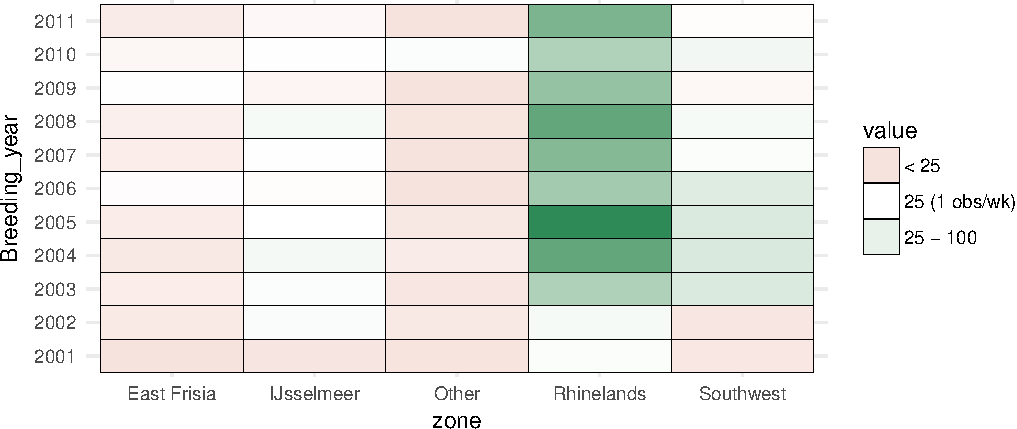
\includegraphics{goose_code008pres_files/figure-beamer/tilemap_space_time-1.pdf}
\caption{Sampling times in each region. Sampling is not even over
zones.}
\end{figure}

\end{frame}

\begin{frame}{Global flock size trend}

\begin{figure}[htbp]
\centering
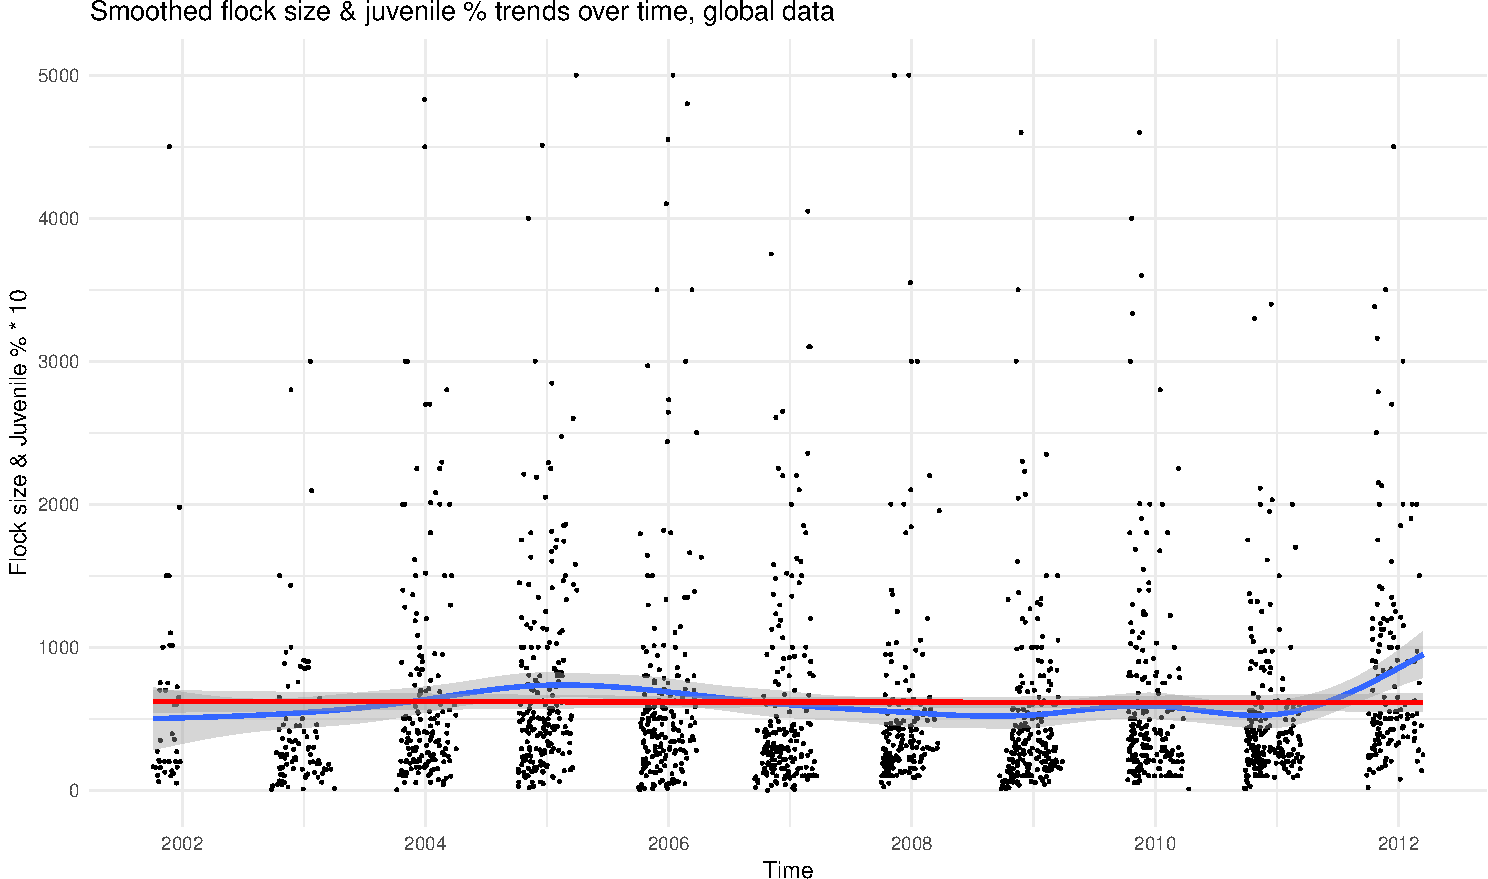
\includegraphics{goose_code008pres_files/figure-beamer/trend_flock_juv_global-1.pdf}
\caption{Global flock size trend follows the lemming cycle.}
\end{figure}

\end{frame}

\begin{frame}{Zonal flock size trend}

\begin{figure}[htbp]
\centering
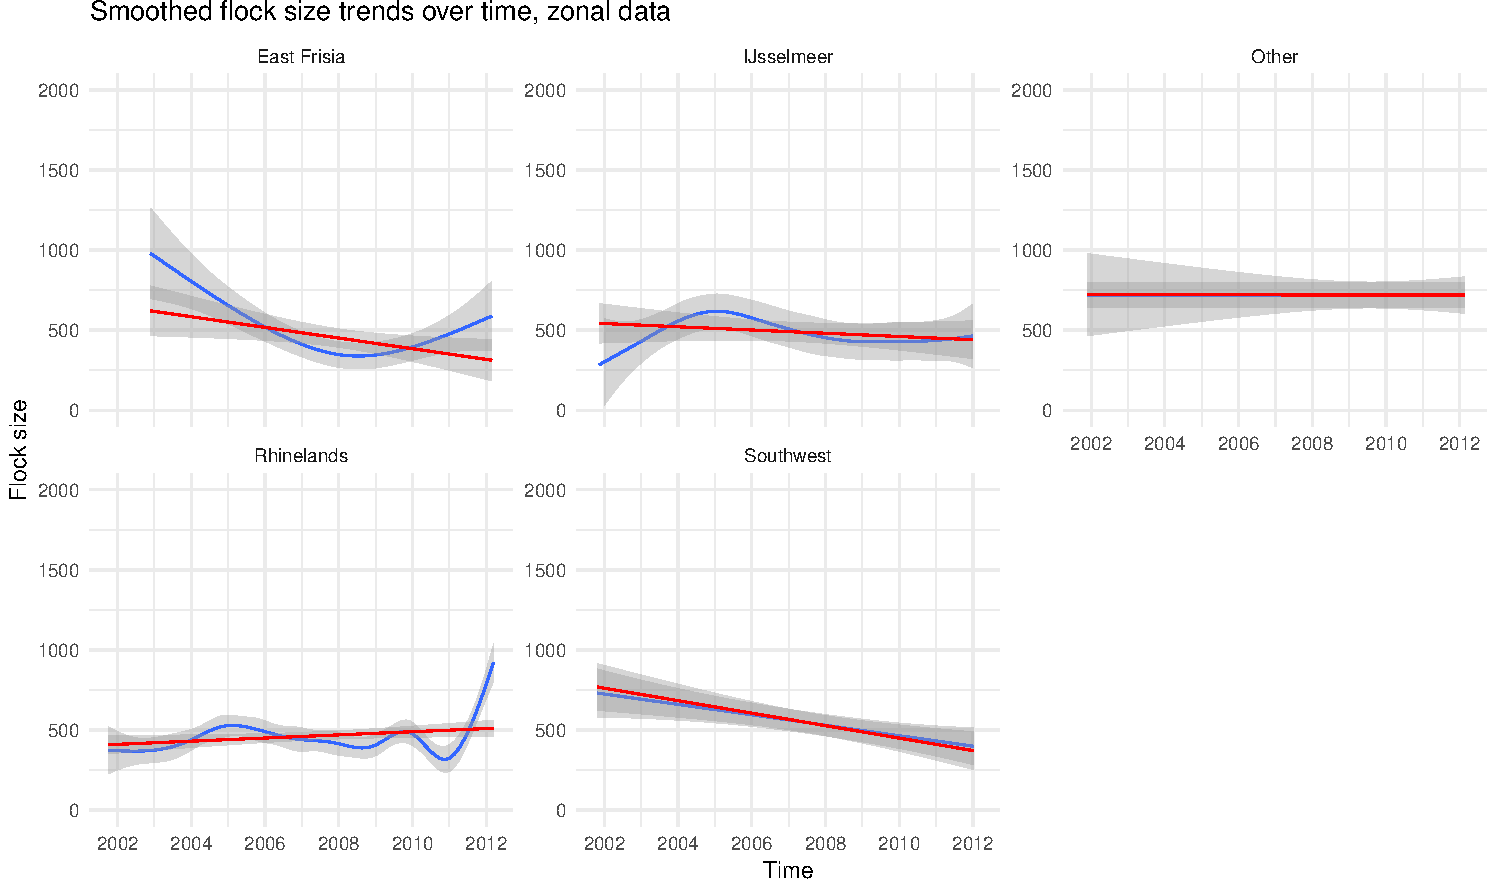
\includegraphics{goose_code008pres_files/figure-beamer/trend_flock_juv_zonal-1.pdf}
\caption{Rhinelands drive the global flock size trend. GAM smoothing:
blue, linear trend: red.}
\end{figure}

\end{frame}

\begin{frame}{Global juvenile \% trend}

\begin{figure}[htbp]
\centering
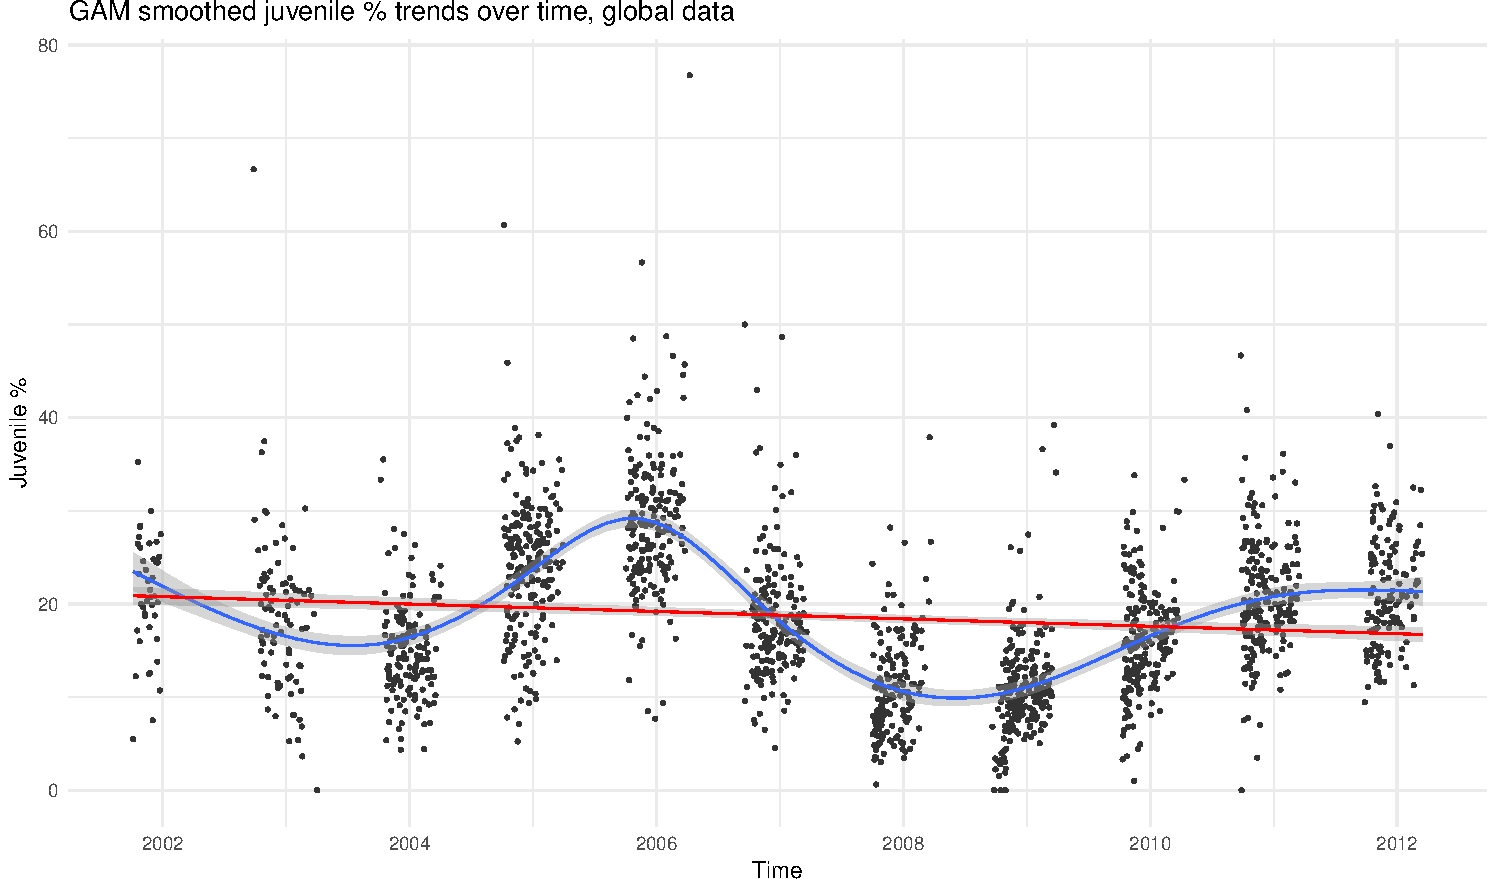
\includegraphics{goose_code008pres_files/figure-beamer/trend_juv_global-1.pdf}
\caption{Global juvenile \% trend also follows lemming cycle. GAM
smoothing, blue; linear trend, red.}
\end{figure}

\end{frame}

\begin{frame}{Zonal juvenile \% trend}

\begin{figure}[htbp]
\centering
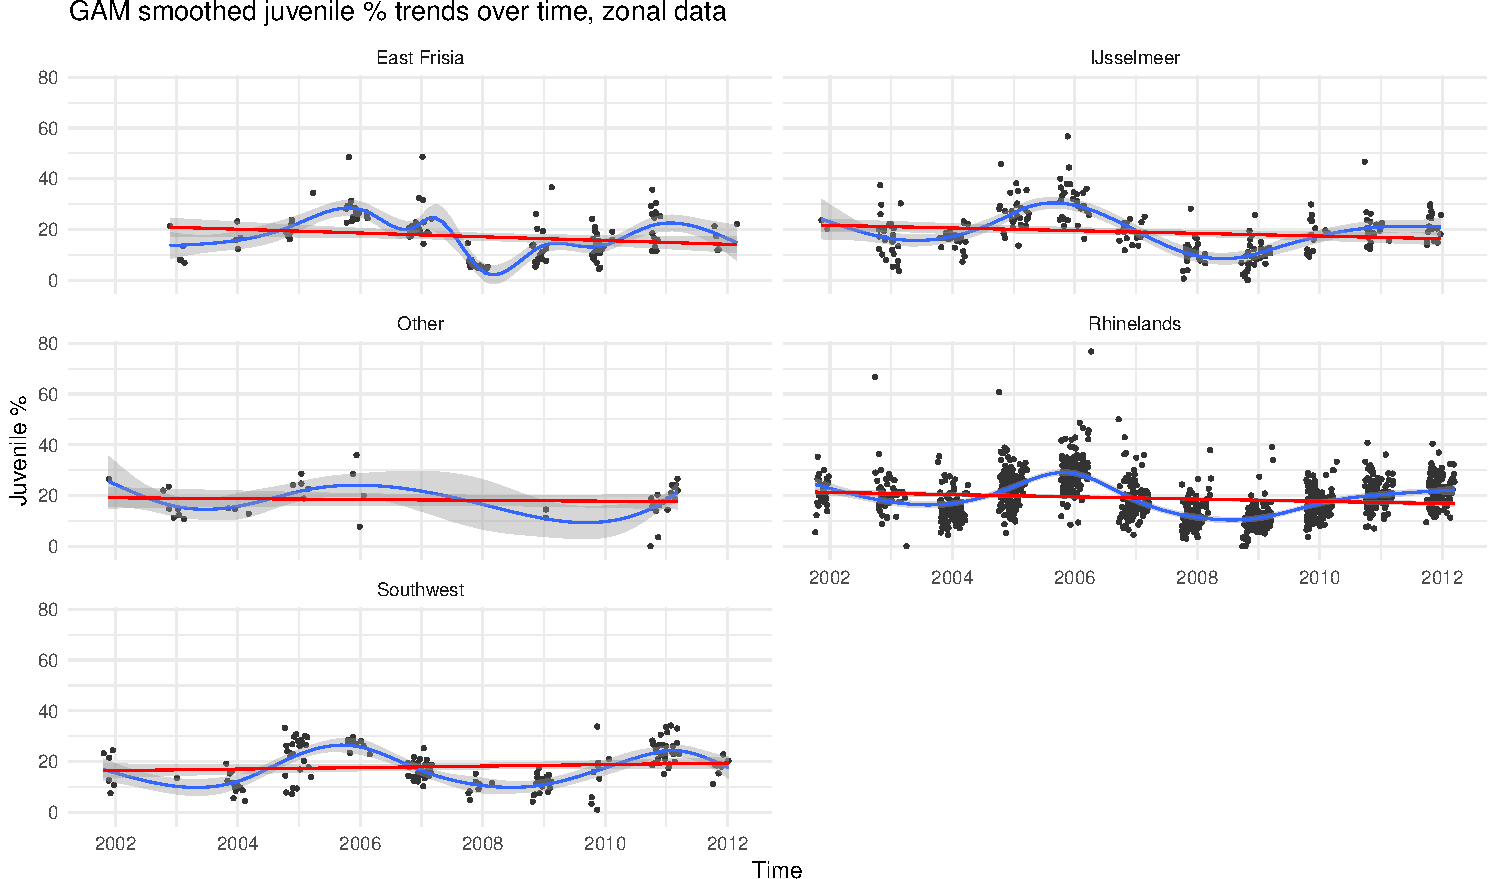
\includegraphics{goose_code008pres_files/figure-beamer/trend_juv_zonal-1.pdf}
\caption{Zonal juvenile \% trends are similar.}
\end{figure}

\end{frame}

\begin{frame}{Global flock size within years}

\begin{figure}[htbp]
\centering
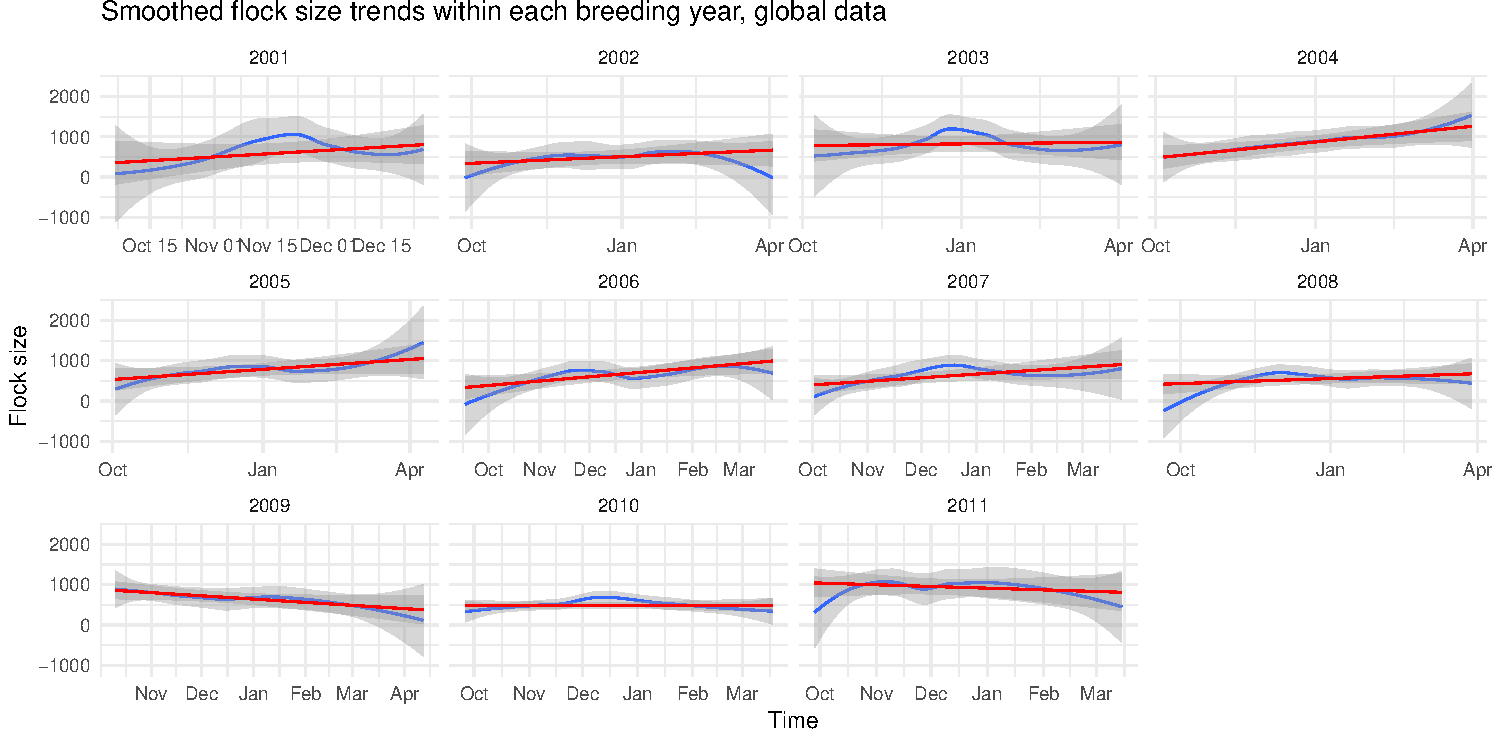
\includegraphics{goose_code008pres_files/figure-beamer/trend_flock_yearly-1.pdf}
\caption{Global flock size trend within years is unrelated to lemming
cycle. Loess smoothing, blue; linear trend, red.}
\end{figure}

\end{frame}

\begin{frame}{Global juvenile \% within years}

\begin{figure}[htbp]
\centering
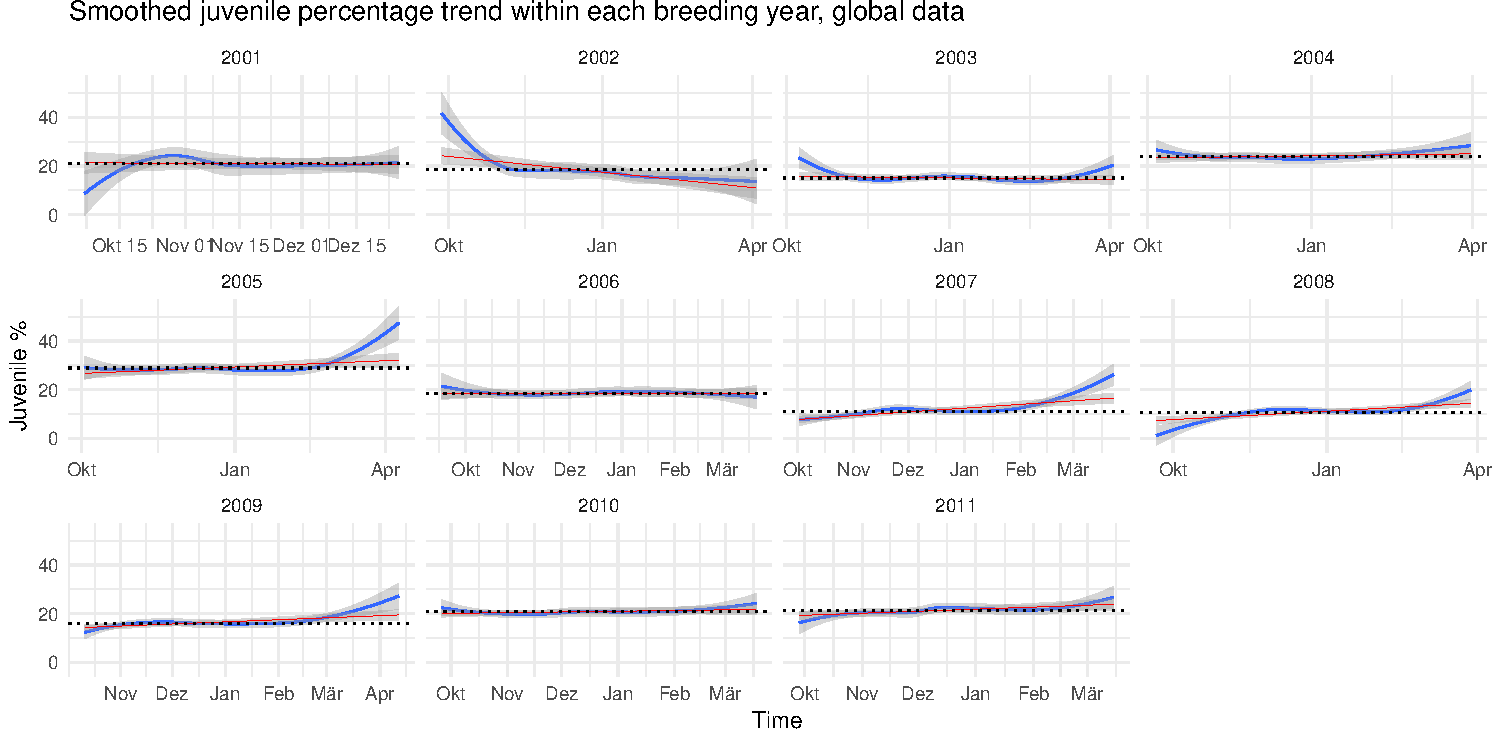
\includegraphics{goose_code008pres_files/figure-beamer/trend_juvprop_yearly-1.pdf}
\caption{Global juvenile \% rises over the winter. Loess smoothing,
blue; linear trend, red; mean \%, dotted line.}
\end{figure}

\end{frame}

\begin{frame}{Family size trend}

\begin{figure}[htbp]
\centering
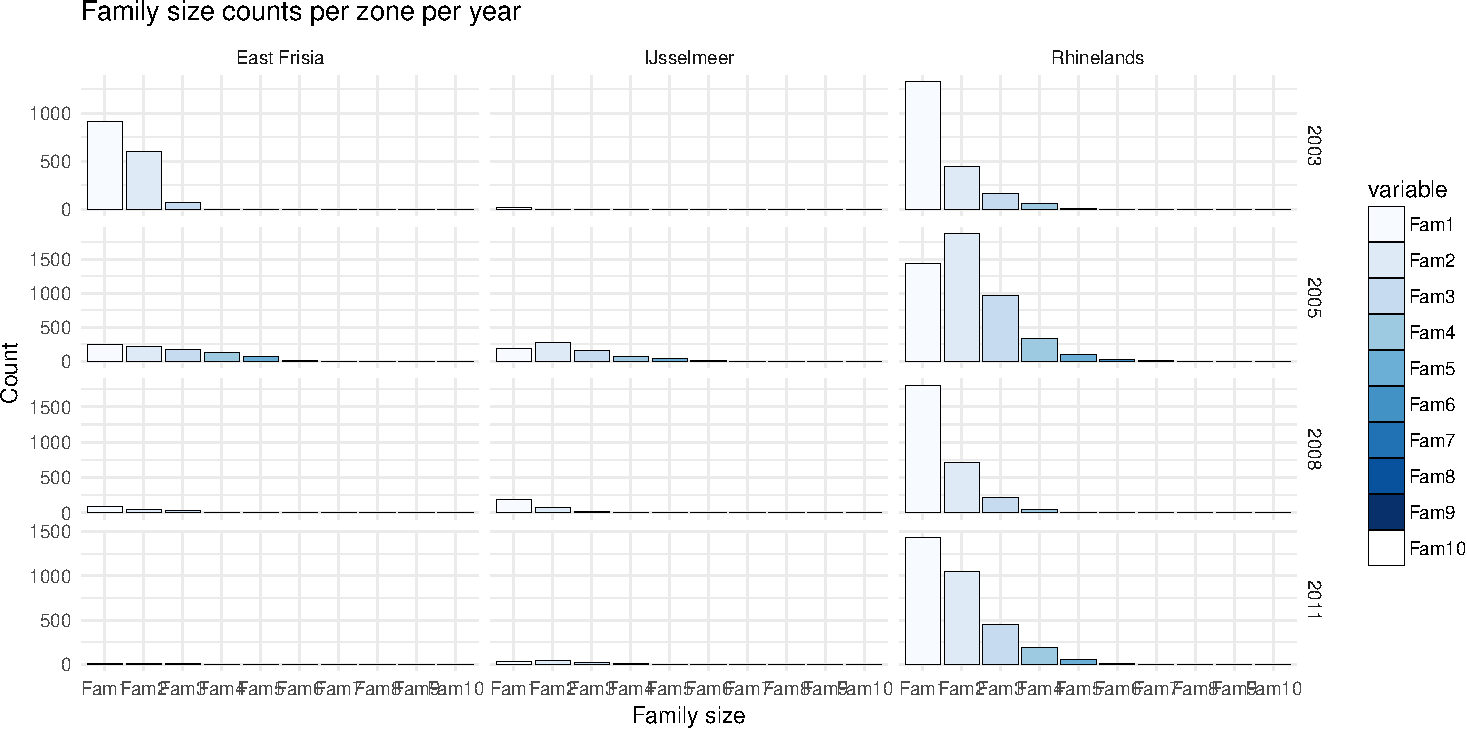
\includegraphics{goose_code008pres_files/figure-beamer/plot_fams_per_year_perzone_persize-1.pdf}
\caption{Families of size \emph{n} are distributed similarly across
zones. Fam2 more in lemming-peak year (2005), less in crash years ('03,
'08).}
\end{figure}

\end{frame}

\begin{frame}{Number of families \textasciitilde{} number of juveniles}

\begin{figure}[htbp]
\centering
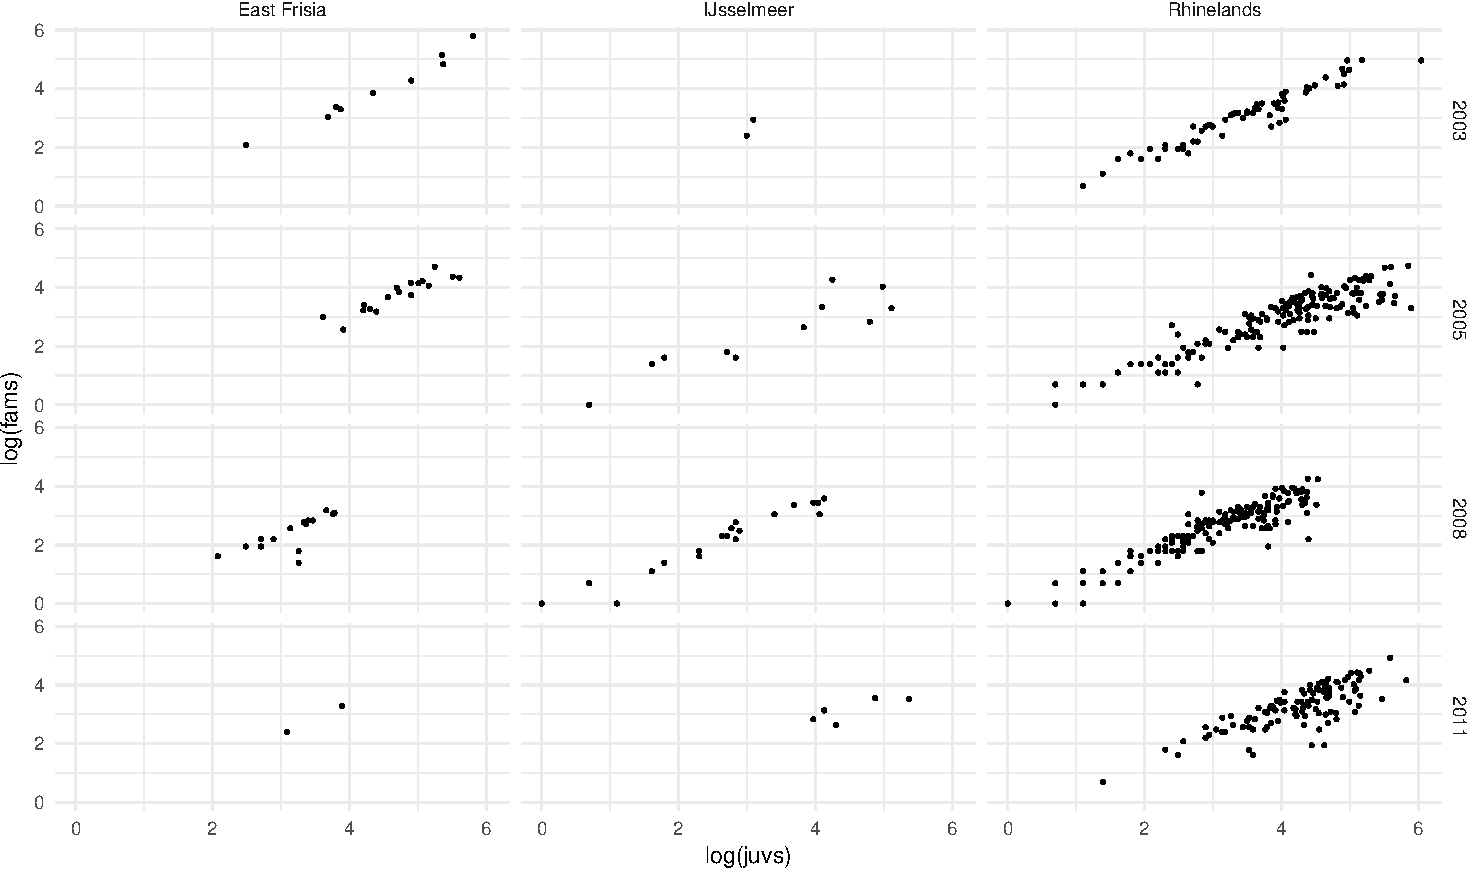
\includegraphics{goose_code008pres_files/figure-beamer/loglogfamsjuvs-1.pdf}
\caption{Total families \textasciitilde{} juvenile count is a linear
relationship on log-log axes.}
\end{figure}

\end{frame}

\begin{frame}{Predicting number of families}

\begin{figure}[htbp]
\centering
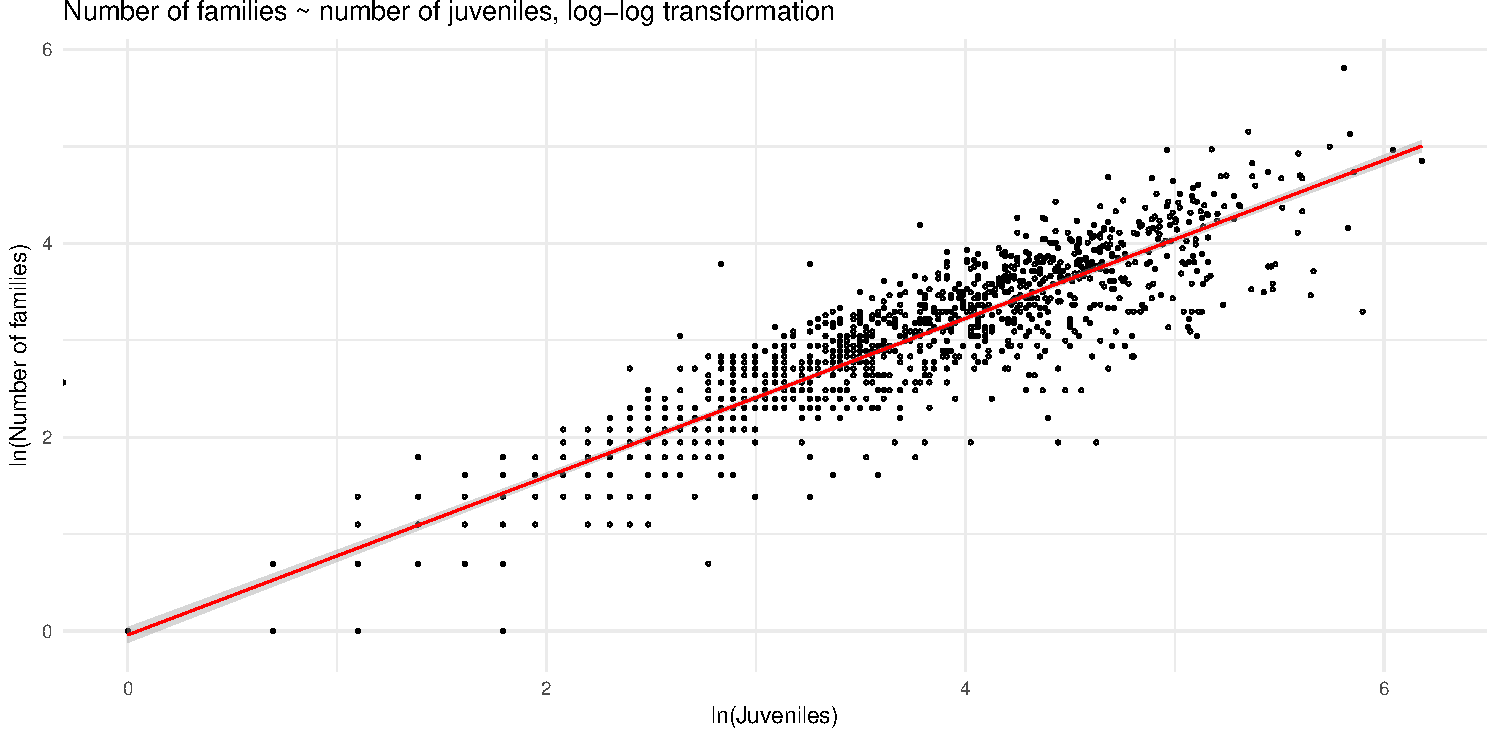
\includegraphics{goose_code008pres_files/figure-beamer/scatterplot_lm1_fams_juvs-1.pdf}
\caption{Model fit and data. Adj. R-squared = 0.83. Possible to get sum
families from juvenile count.}
\end{figure}

\end{frame}

\begin{frame}

\begin{figure}[htbp]
\centering
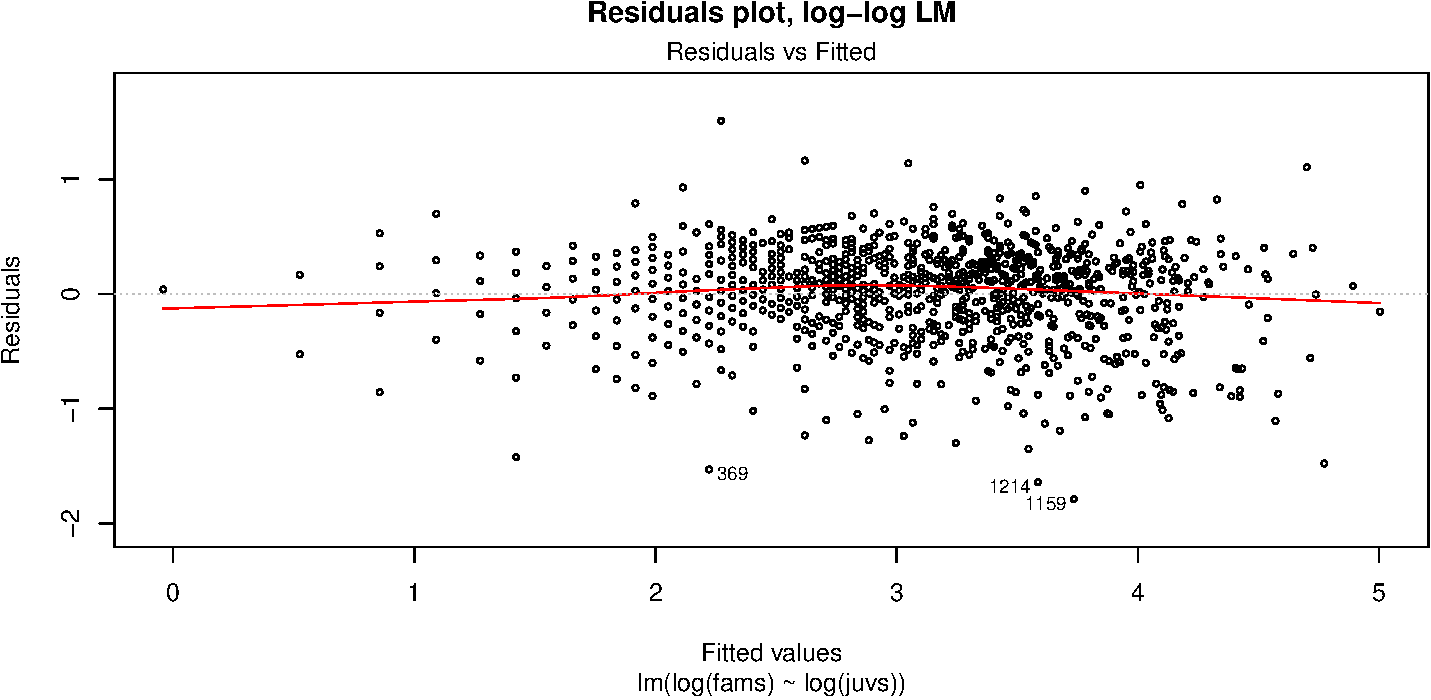
\includegraphics{goose_code008pres_files/figure-beamer/compare_nls_lm_resids-1.pdf}
\caption{Linear model residual plot.}
\end{figure}

\end{frame}

\end{document}
